\documentclass[usenames,dvipsnames,tikz]{standalone}
\usepackage{xcolor}
\colorlet{tBlue}{RoyalBlue!35!Cerulean}
\colorlet{tRed}{Red}
\usepackage{tikz}
\usepackage{standalone}
\begin{document}
	
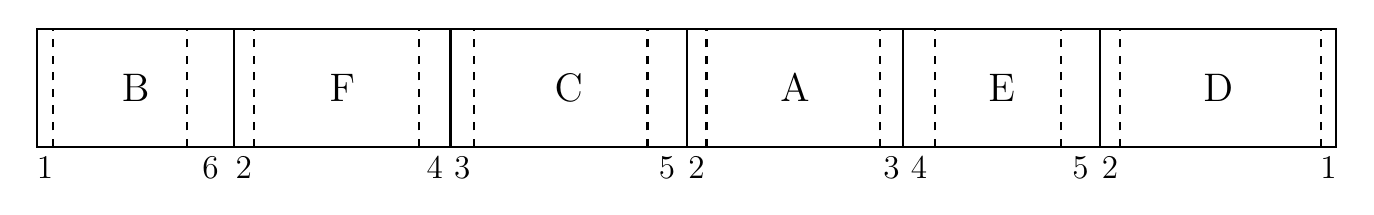
\begin{tikzpicture}
%\draw [help lines] (-1,-2) grid (17.5,4);

\draw [thick] (0,0) rectangle (16.5,1.5); %whole rectangle
\draw [thick] (2.5,0) -- (2.5, 1.5); % between B and F
\draw [thick] (5.25,0) -- (5.25, 1.5); % between F and C
\draw [thick] (8.25,0) -- (8.25, 1.5); % between C and A
\draw [thick] (11,0) -- (11, 1.5); % between A and E
\draw [thick] (13.5,0) -- (13.5, 1.5); % between E and D

\draw [thick, dashed] (0.2,0) -- (0.2, 1.5);
\draw [thick, dashed] (1.9,0) -- (1.9, 1.5);
\draw [thick, dashed] (2.75,0) -- (2.75, 1.5);
\draw [thick, dashed] (4.85,0) -- (4.85, 1.5);
\draw [thick, dashed] (5.55,0) -- (5.55, 1.5);
\draw [thick, dashed] (7.75,0) -- (7.75, 1.5);
\draw [thick, dashed] (8.5,0) -- (8.5, 1.5);
\draw [thick, dashed] (10.7,0) -- (10.7, 1.5);
\draw [thick, dashed] (11.4,0) -- (11.4, 1.5);
\draw [thick, dashed] (13,0) -- (13, 1.5);
\draw [thick, dashed] (13.75,0) -- (13.75, 1.5);
\draw [thick, dashed] (16.3,0) -- (16.3, 1.5);

\node [below] at (0.1, 0) {\large{1}};
\node [below] at (2.2, 0) {\large{6}};
\node [below] at (2.625, 0) {\large{2}};
\node [below] at (5.05, 0) {\large{4}};
\node [below] at (5.4, 0) {\large{3}};
\node [below] at (8, 0) {\large{5}};
\node [below] at (8.375, 0) {\large{2}};
\node [below] at (10.85, 0) {\large{3}};
\node [below] at (11.2, 0) {\large{4}};
\node [below] at (13.25, 0) {\large{5}};
\node [below] at (13.625, 0) {\large{2}};
\node [below] at (16.4, 0) {\large{1}};

\node at (1.25,0.75) {\Large{B}};
\node at (3.875,0.75) {\Large{F}};
\node at (6.75,0.75) {\Large{C}};
\node at (9.625,0.75) {\Large{A}};
\node at (12.25,0.75) {\Large{E}};
\node at (15,0.75) {\Large{D}};




\end{tikzpicture}
\end{document}